% Report insert for Sections 3--5. Compile from the repository root.
% Required packages in the main preamble: graphicx, booktabs, tabularx.

% --- Section 3: Work Completed ---
\section*{3. Work Completed}
\subsection*{Simulation setup and comparison design}

I used the current public repository's paper-specific, infinite-horizon
scenarios to examine Figures 6--7. I configured the fixed
\texttt{gpt-4o-2024-11-20} model with temperature 0 and seed 42, and ran
the \$56 and \$14 initial-price cases against a \$28 fundamental value.
Each case involved eight agents over 15 rounds and produced 120
successful agent decisions. I then repeated both cases after clarifying
the market makers' inventory constraint in their system prompt, while
retaining the scenario parameters and market rules. For all four runs,
I preserved the rendered prompts and examined orders, trades, recorded
prices, and reported agent valuations. The prompt comparison is
exploratory because the paired runs did not realize identical dividend
paths.

% --- Section 4: Preliminary Findings ---
\subsection*{Figure 6--7 replication: price formation and agent valuations}

I examined the paper's two infinite-horizon price-discovery scenarios
using the current public codebase. Each scenario has eight LLM agents,
15 trading rounds, and a fundamental value of \$28. The original
starting prices are \$56 and \$14. The results below refer to my
seed-42 runs; they are separate from other runs summarized elsewhere
in this joint report. Both scenarios completed 120 successful agent
decisions. I also changed only the market makers' system-prompt wording
to clarify that they could sell only shares they owned, then reran
both scenarios. Table~\ref{tab:my-fig6-results} summarizes the results.

\begin{table}[htbp]
\centering
\small
\caption{My Figure 6 runs. ``End price'' is the simulator's recorded
price, which can change without a trade. Buy/Sell counts are accepted
orders; volume counts executed shares. Gap closed is the reduction in
the absolute distance from \$28 divided by the initial distance.}
\label{tab:my-fig6-results}
\begin{tabular}{@{}lrrrrr@{}}
\toprule
\textbf{Run} & \textbf{End price} & \textbf{Trades} &
\textbf{Volume} & \textbf{Buy/Sell} & \textbf{Gap closed} \\
\midrule
\$56 baseline        & \$46.00 & 0  & 0      & 0/103   & 35.7\% \\
\$56 prompt adjusted & \$50.40 & 0  & 0      & 0/120   & 20.0\% \\
\$14 baseline        & \$15.35 & 23 & 13,999 & 172/17  &  9.6\% \\
\$14 prompt adjusted & \$15.30 & 24 & 22,000 & 123/40  &  9.3\% \\
\bottomrule
\end{tabular}
\end{table}

Figure~\ref{fig:my-fig6-comparison} places the paper's Figure 6
panels alongside the price paths from my runs. The paper reports
persistent overpricing from \$56 and marked convergence toward \$28
from \$14 (Lopez-Lira, 2025, Sec.~3.2.3). In my \$56 runs, every
accepted order was a sell and no trade executed. The recorded-price
decline to \$46.00 or \$50.40 therefore reflects the current code's
order-book quote fallback, not transaction-based price discovery.
In my \$14 runs, actual trades occurred, but the price ended near
\$15, far from \$28. Changing the market-maker prompt did not resolve
either mechanism. Because the baseline and prompt-adjusted runs had
different realized dividend paths, their endpoint differences cannot
be attributed solely to the wording change.

\begin{figure}[htbp]
\centering
\begin{tabular}{@{}cc@{}}
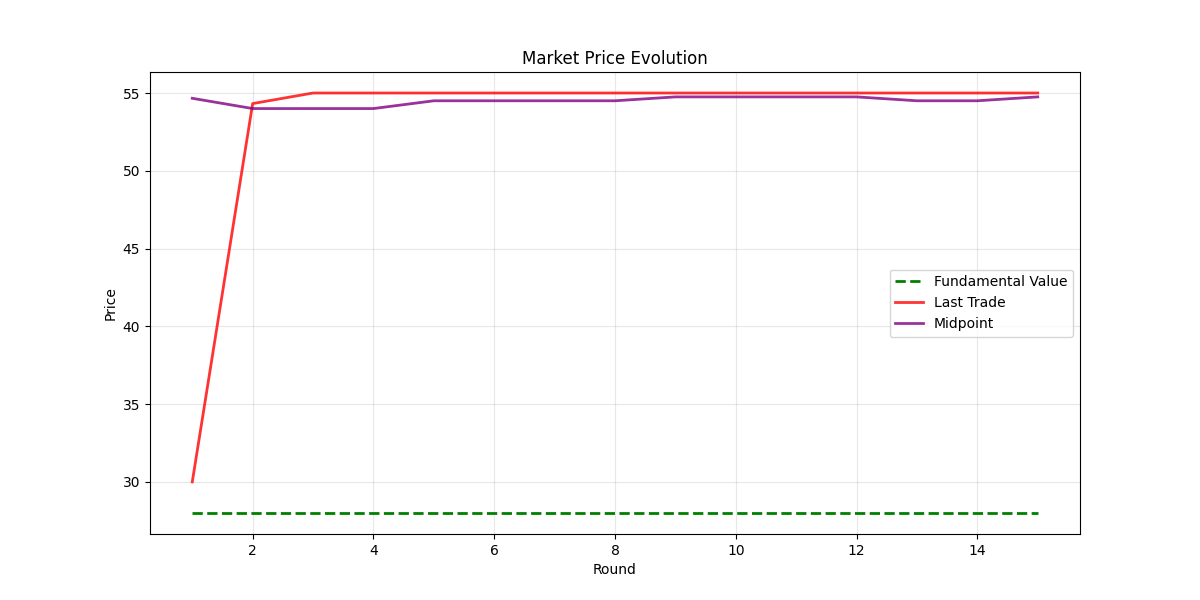
\includegraphics[width=.47\textwidth]{docs/figures/paper_fig6_above.png} &
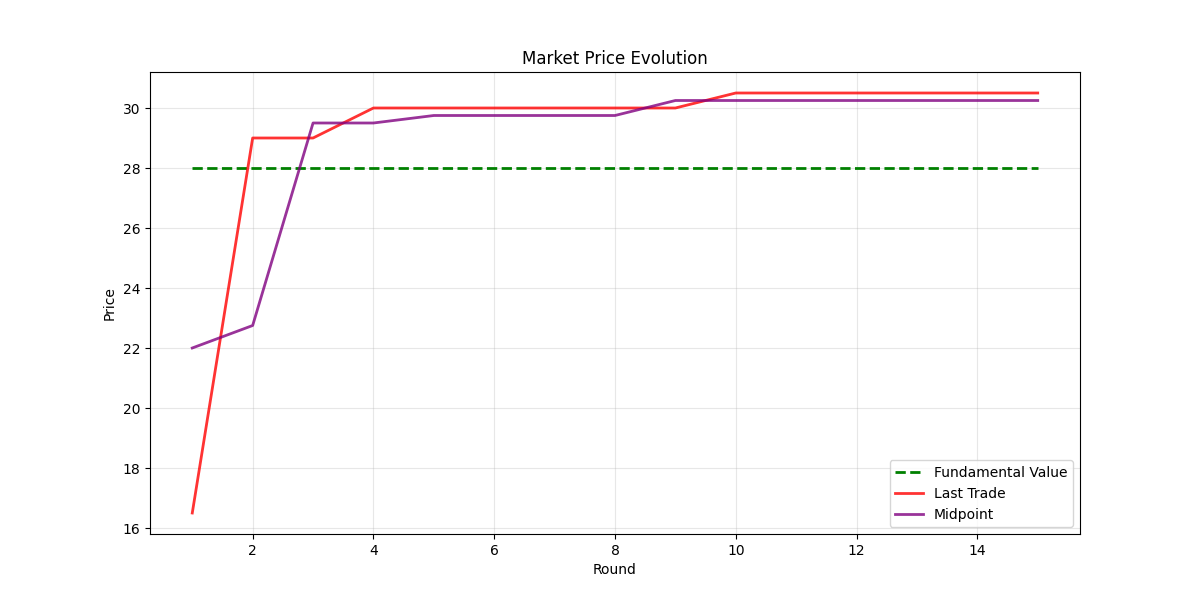
\includegraphics[width=.47\textwidth]{docs/figures/paper_fig6_below.png} \\
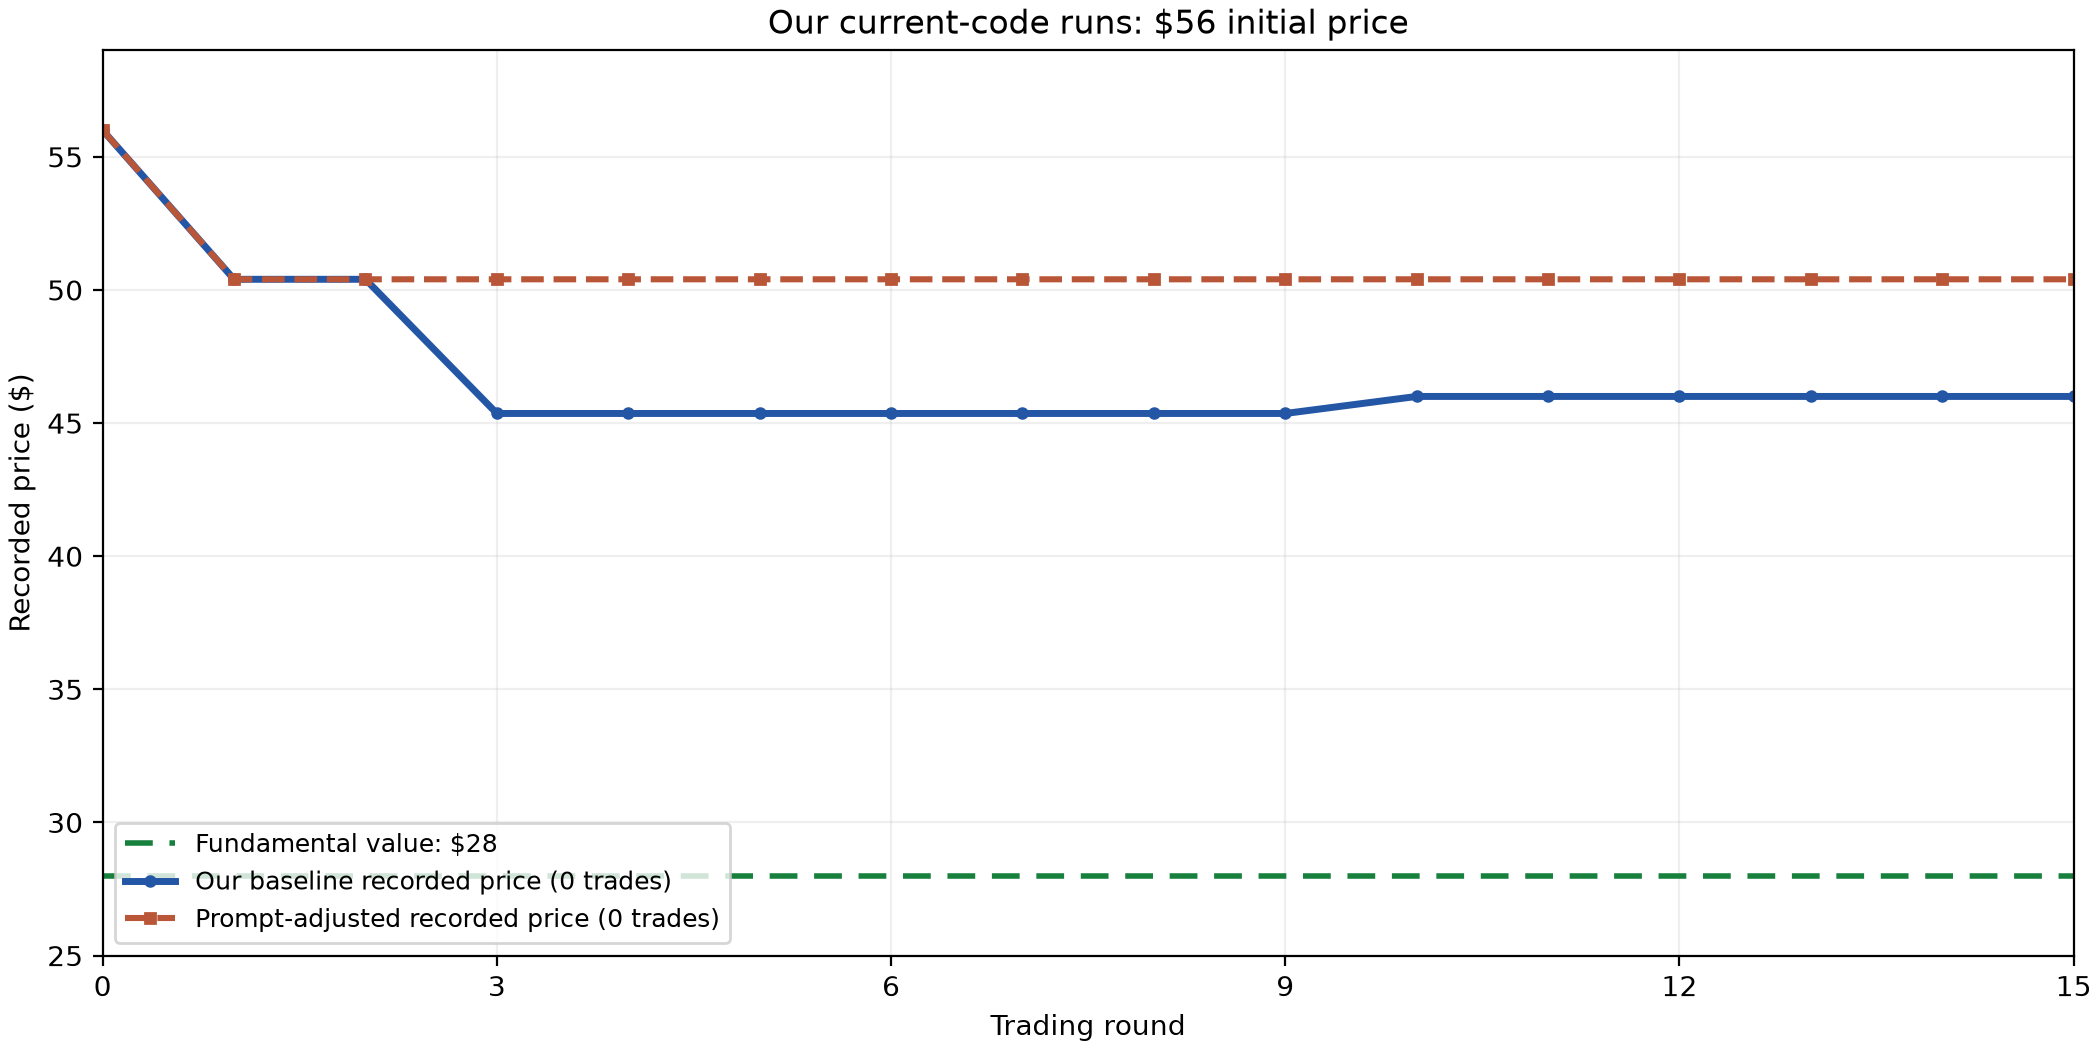
\includegraphics[width=.47\textwidth]{docs/figures/ours_fig6_above.png} &
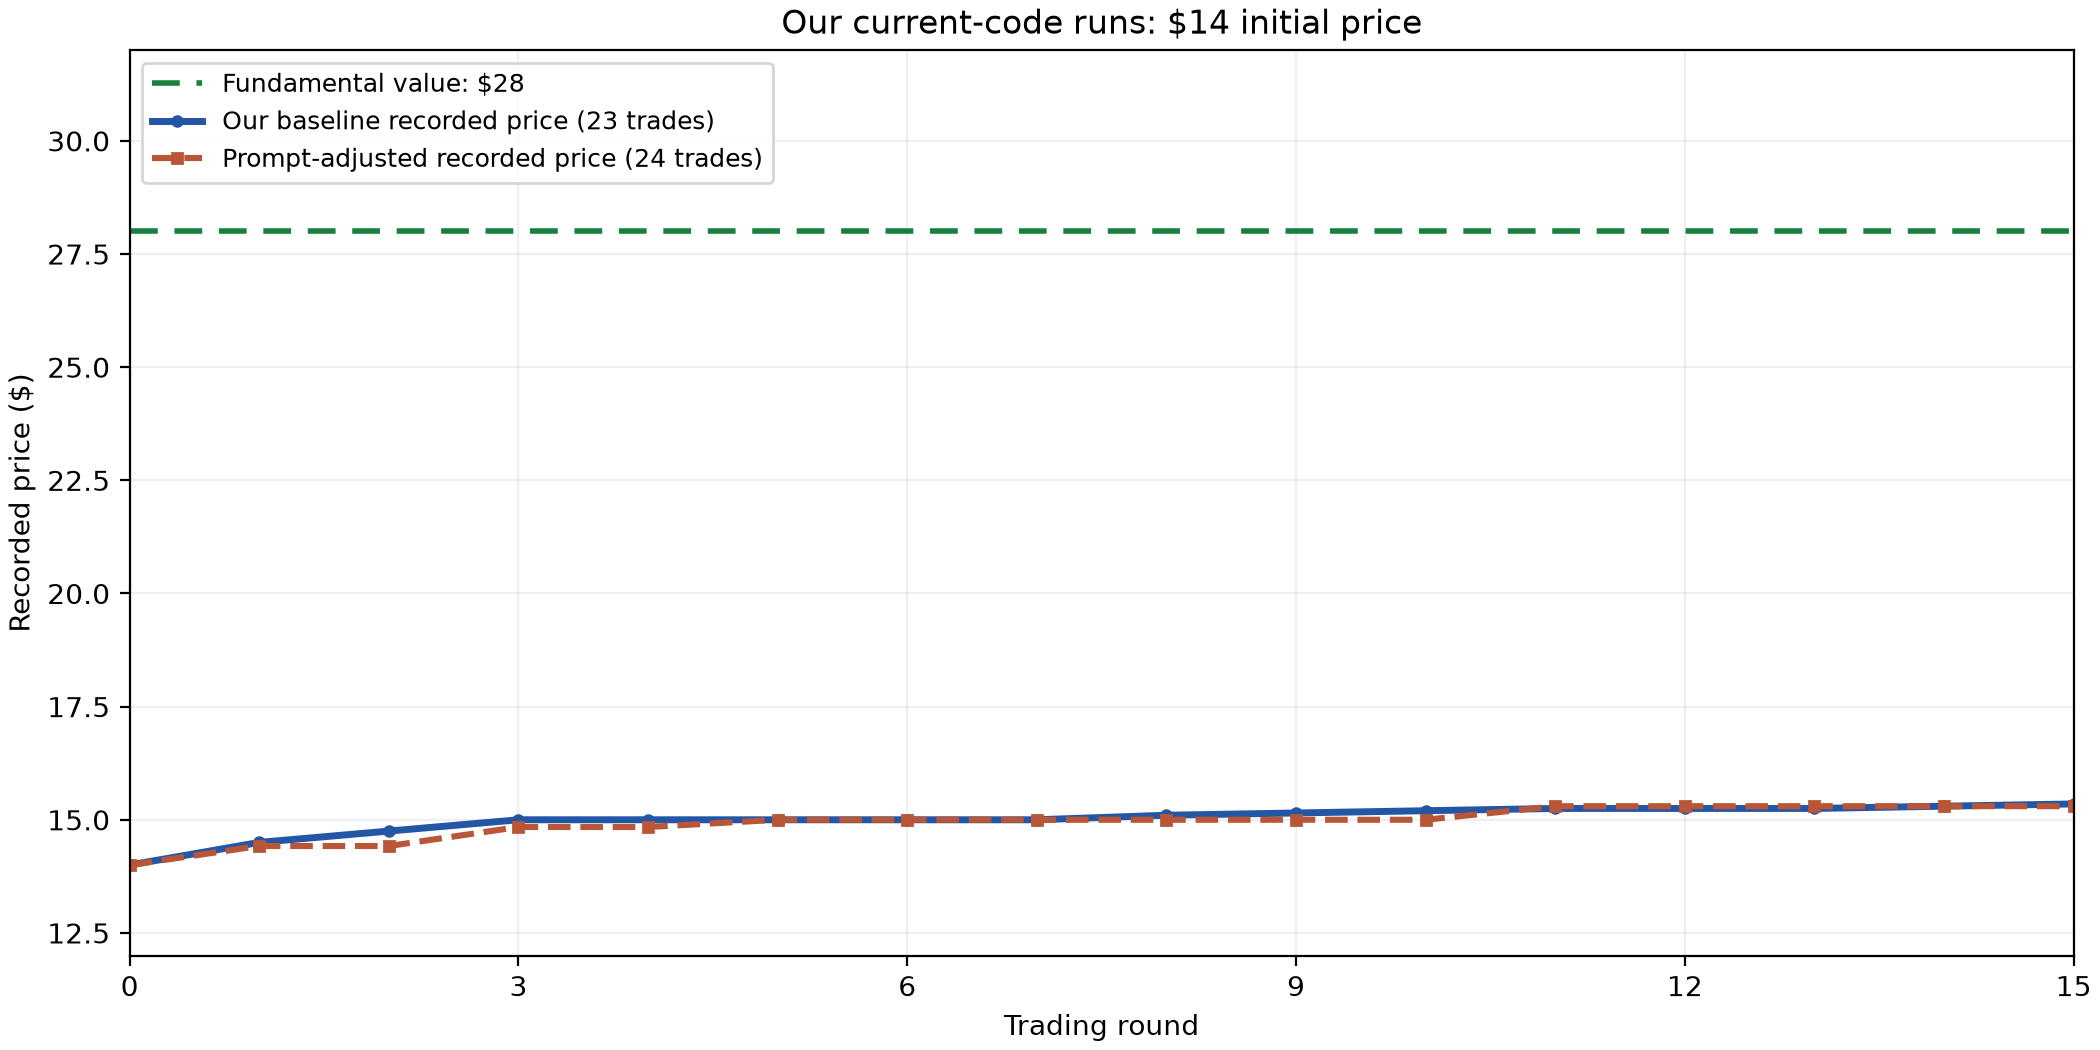
\includegraphics[width=.47\textwidth]{docs/figures/ours_fig6_below.png}
\end{tabular}
\caption{Figure 6 comparison. Top: published plots for the \$56 and
\$14 starting prices, reproduced from Lopez-Lira (2025), Figure 6.
They label last trade and midpoint. Bottom: my current-code baseline
and prompt-adjusted runs; these plots show the simulator's recorded
price, so the series are not yet the same price measure. The \$56
runs had no executed trades and no two-sided midpoint.}
\label{fig:my-fig6-comparison}
\end{figure}

The valuation comparison for Figure 7 is also different from the
paper's description. Table~\ref{tab:my-fig7-results} uses the
baseline runs; these are agents' reported valuations, not inferred
values from their executed orders.

\begin{table}[htbp]
\centering
\small
\caption{Figure 7: published description versus my baseline runs.}
\label{tab:my-fig7-results}
\begin{tabularx}{\textwidth}{@{}lXX@{}}
\toprule
\textbf{Start} & \textbf{Paper's description} & \textbf{My observation} \\
\midrule
\$56 & Several agent valuations stay above the \$28 fundamental. &
The round-wise median is \$28 throughout; six agents report \$28
and two optimistic agents report \$41.60. \\
\$14 & Valuations adjust upward toward \$28. &
The round-wise median is already \$28 in round 1 and remains there;
the two optimistic agents report \$40.00 or \$41.60. \\
\bottomrule
\end{tabularx}
\end{table}

These are single-run comparisons with the present repository. The
paper's exact Figure 6--7 code version, rendered prompts, and raw
plotting data have not been identified. The public repository belongs
to the paper's author, but its first visible commit postdates the
paper's submission.

% --- Section 5: Next Steps ---
\subsection*{Resolving the Figure 6--7 replication gap}

\begin{enumerate}
\item \textbf{Establish comparability.} Check historical code and prompts
against the paper, and seek the original figure data if available.
Reconstruct last-trade prices and two-sided midpoints from the logs;
label rounds with no trade or no midpoint rather than treating the
simulator's recorded price as an executed price.

\item \textbf{Identify the trading mechanism.} Trace accepted and
rejected orders, quotes, market-maker decisions, and agent valuations
to explain the absence of buyers at \$56 and weak upward movement
from \$14.

\item \textbf{Test sensitivity and robustness.} After controlling
dividend and order-sequencing randomness, repeat a small matched set
of seeds and test \$35/\$21 as a separate 15-round infinite-horizon
sensitivity analysis, holding agent composition and market rules
fixed. This is not the paper's 20-round finite-horizon experiment.
\end{enumerate}

For the next meeting, the priority is to explain the baseline results
and provide an initial robustness check.

\subsection*{Beyond Figure 6--7}

\begin{enumerate}
\item \textbf{Near term: agent-level behavior.} Use existing decision
logs, then controlled price-to-fundamental tests, to examine strategy
adherence, order choice, and valuation responses as in Figures 2--5.

\item \textbf{Later term: AI herding.} Once the baseline is understood,
compare similar and diverse agent prompts or compositions. Measure
decision alignment separately from market effects such as trading
volume, liquidity, and price impact; treat this as a new mechanism
test, not a Figure 6--7 replication.
\end{enumerate}
